\section{Design Space}
\label{sec:dspace}

The narrow interface exposed by storage systems has been a boon in allowing
systems and applications to evolve independently, in affect limiting the size
of the design space where applications couple with storage. Programmable
storage lifts the veil on the system, and with it, forces applications developers
to confront a large set of possible designs.

\subsection{Software Parameters}

To illustrate the design space challenge we implemented as an object interface
the CORFU storage device specification, that is a write-once interface over a
64-bit address space. The interface is used as a building block of the CORFU
protocol to read and write log entries that are striped over an entire
cluster.  The implementations differ in their optimization strategy of
utilizing internal system interfaces. For instance one implementation uses a
key-value interface to manage the address space index and entry data, while
another implementation stores the entry data using a byte-addressable
interface.

\begin{figure}[t]
\centering
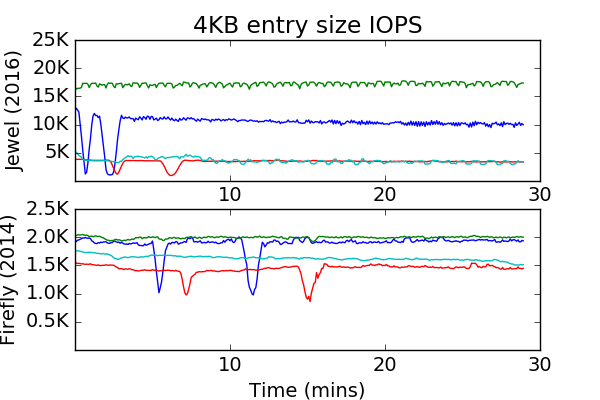
\includegraphics[width=1.0\linewidth]{jewel_v_firefly_pd.png}
\caption{Relative performance differences can be drastic after a software
    upgrade of the underlying storage system.}
\label{fig:phy-design}
\end{figure}

Figure~\ref{fig:phy-design} shows the append throughput of four such
implementations run on two versions of Ceph from 2014 and 2016. The first
observation to be made is that performance in general is significantly better
in the newer version of Ceph. However, what is interesting is the relationship
between the implementations. Run on a version of Ceph from 2014, the top two
implementations perform with nearly identical throughput, but have strikingly
different implementation complexities. The performance of the same
implementations on a newer version of Ceph illustrate a challenge: given a
reasonable choice of a simpler implementation in 2014, a storage interface
will perform worse in 2016, requiring significant rework of low-level
interface implementations.

\textbf{Takeaway}: Choosing the best implementations is dependent on both the
timing of the development (Ceph Version) and the expertise of the
administrator (Ceph Features). Ceph development is a moving target with
multiple stable releases each year, 400+ contributors, and 70--260 commits per
week.  Disruptive and innovative change in Ceph is also common place, with
features such as BlueStore~\cite{weil:vault2016-bluestore} replacing
traditional file systems like XFS that have limitations on the workloads
generated by Ceph such as double writes and metadata scalability. 

\subsection{System Tunables}

A recent version of Ceph (v10.2.0-1281-g1f03205) has 994 tunable
parameters, where 195 of them pertain to the object server itself
and 95 of them focus on low-level storage abstractions built on XFS or
BlueStore. Ceph also has tunables for the subsystems it uses, like
LevelDB (10 tunables), RocksDB (5 tunables), its own key-value stores (5
tunables), its object cache (6 tunables), its journals (24 tunables), and its
other optional object stores like BlueStore (49 tunables).
Auto-tuning~\cite{behzad:sc2013-autotuning} techniques have been applied to
systems with a large space of parameters with limited success, but the
challenge is exacberated in the context of application-specific modifications
and workloads that change dynamically. Next we show an example of an
application-specific optimization technique that benefits from dynamic tuning.

\subsubsection{Application-specific Group Commit}

Group commit is a technique used in database query execution that combines
multiple transactions in order to amatorize over per-transaction fixed costs
like logging. Figure~\ref{fig:batching} shows the performance impact of using
a \emph{group commit}-like technique for combining log appends from
independent clients into a single request.  The \emph{simple} case implements
group commit at the request level, but processes each sub-request append
indepently using low-level I/O interfaces. The modest performance increase is
attributed to a reduction in average per-request costs related to network
roundtrips. Compared with the \emph{simple} case, the \emph{batching-aware}
the \emph{batch-aware} implementation is able to achieve significantly higher
performance by constructing more efficient I/O requests using range queries
and data sieving techinques provided by the low-level I/O interfaces.

\begin{figure}
\centering
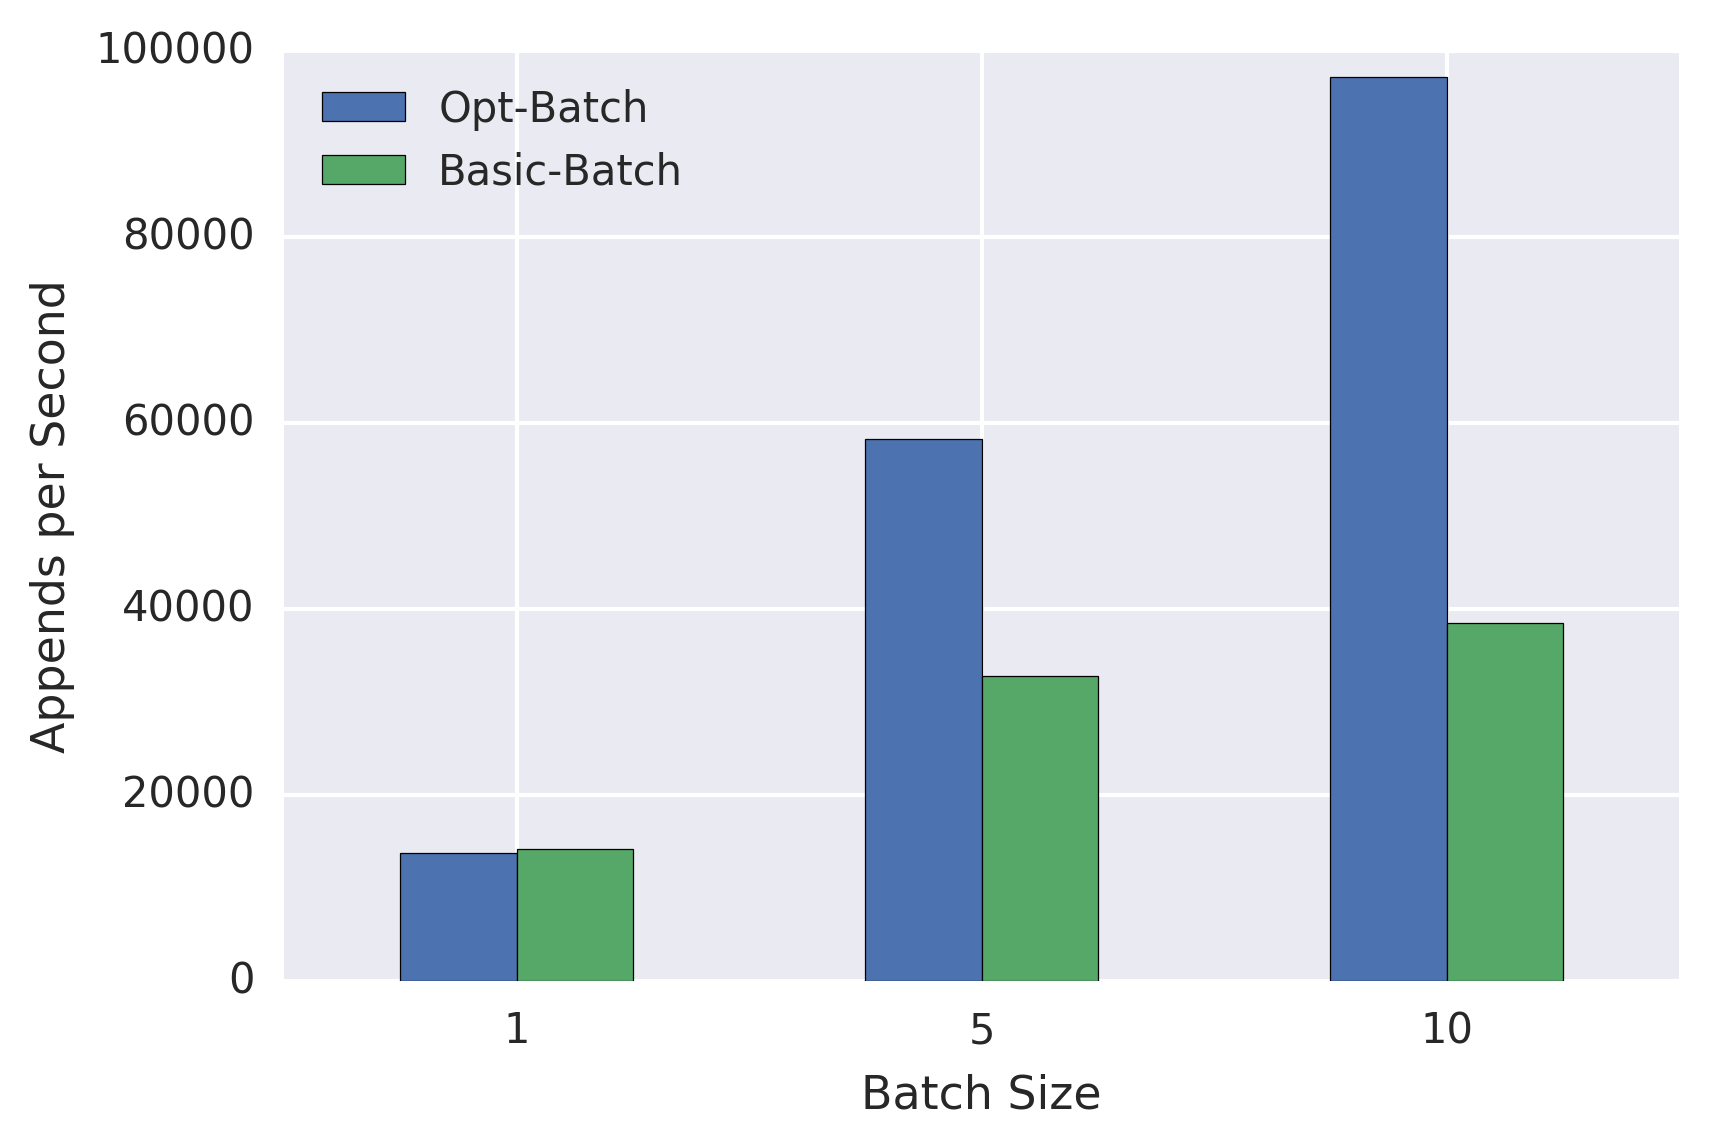
\includegraphics[width=1.0\linewidth]{batching.png}
\caption{Total throughput with and without batching.}
\label{fig:batching}
\end{figure}

The batched execution technique of group commit can significantly increase
throughput, but the story is much more complex. The ability to apply this
techinque requires tuning parameters such as adding artifical delays to
increase batch size that will also affect latency, and parameter tuning is
affected dynamically by workload patterns.  While the performance impact of
application-specific batching is significant, techniques such as range queries
and data sieving are sensitive to outliers that can occur with buggy or slow
clients.

When outliers occur in a batch, naively building large I/O requests can result
in a large amount of wasted I/O.  Figure~\ref{fig:batching-outlier} highlights
this scope of this challenge. The \emph{simple} case handles each request in
the batch independently, and while it performs relatively worse than the other
techniques, it is not sensitive to outliers. The \emph{batch-aware}
implementation achieves high append throughput, but performance degrades as
the magnitude of the batch outlier increases. In contrast, the
\emph{batch-oident} applies a simple heuristic to identify the outlier and
handle it independently, resulting in only a slight decrease in performance
over the best case.

\begin{figure}
\centering
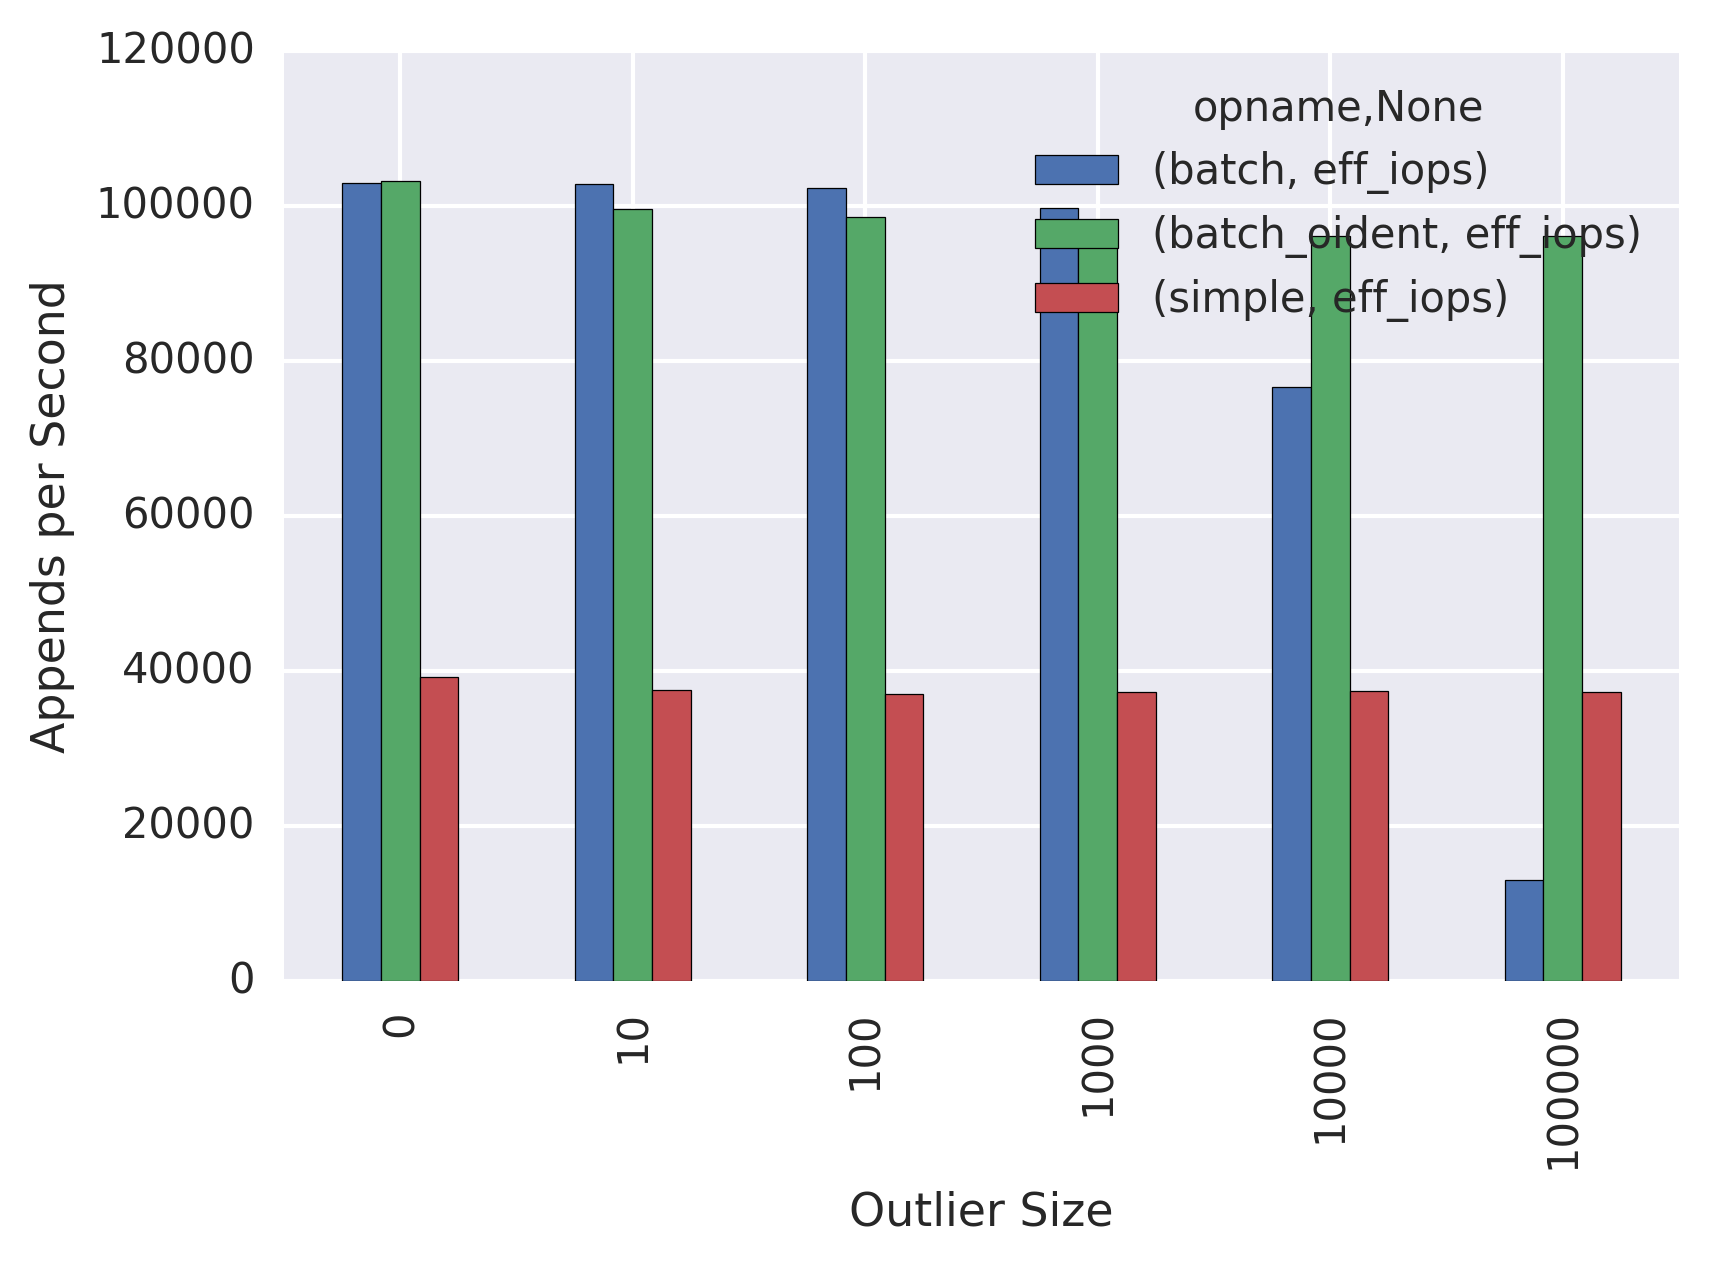
\includegraphics[width=1.0\linewidth]{batching-outlier-detect.png}
\caption{Identifying and handling an outlier independently maintains the
beneifts of batching without the performance degredation of unecessarily
large I/O requests.}
\label{fig:batching-outlier}
\end{figure}

\textbf{Takeaway}: System tunables present a challenge in optimizing systems,
even in static cases with fixed workloads. Programmable storage approaches
that introduce application-specific interfaces that are sensitive to changes
in workloads including adverserial cases that must be analyzed and handled
greatly increase the design space and set of concerns to be addressed.

\subsection{Hardware Parameters}

Ceph is designed to run on a wide variety of commodity hardware as well as new
NVMe devices. All these devices have their own set of characteristics and
tunables (e.g., the IO operation scheduler type). In our experiments, we tested
SSD, HDDs, NVMe devices and discovered a wide range of behaviors and
performance profiles. While we generally observe the expected result of faster
devices resulting in better application performance, choosing the best
implementation strategy is highly dependent on hardware. The changes in Ceph
required to fully exploit the performance profile of NVMe, persistent
memory, and RDMA networks will likely result in new design trade-offs for
application-specific interface designs.
